\documentclass{beamer}

\usepackage[utf8]{inputenc}
\usepackage[T1]{fontenc}
\usepackage[polish]{babel}
\usepackage{minted}

\usetheme{Madrid}

\title[Efektywna reprezentacja słownika]{Efektywna reprezentacja słownika jako minimalny automat deterministyczny}
\subtitle{Biblioteka Lexicon w C++20\\Zaawansowane Biblioteki Programistyczne}
\author{Piotr Marcol}
\date{26.05.2026}

\begin{document}

% Frame 1
\frame{\titlepage}

% Frame 2
\begin{frame}{Plan prezentacji}
    \tableofcontents
\end{frame}

\section{Wprowadzenie i API}

% Frame 3
\begin{frame}{Cel projektu}
    \begin{itemize}
        \item reprezentacja zbioru słów jako minimalny automat deterministyczny,
        \item szybkie sprawdzanie, czy słowo należy do słownika,
        \item ograniczenie redundancji przez współdzielenie prefiksów i sufiksów,
        \item API zbliżone do kontenera STL,
        \item możliwość eksportu struktury do Graphviz DOT.
    \end{itemize}
\end{frame}

% Frame 4
% \begin{frame}{Od teorii do implementacji}
%     \begin{itemize}
%         \item poprzednio: Trie, DAFSA, minimalizacja i przykłady grafów,
%         \item teraz: działająca biblioteka \texttt{lexicon::Lexicon},
%         \item język: C++20,
%         \item wejście: posortowany zbiór słów,
%         \item wynik: zminimalizowany automat gotowy do zapytań.
%     \end{itemize}
% \end{frame}

% Frame 5
\begin{frame}{Struktura projektu}
    \begin{itemize}
        \item \texttt{include/lexicon/lexicon.hpp} -- publiczne API biblioteki,
        \item \texttt{src/lexicon.cpp} -- implementacja automatu,
        \item \texttt{examples/main.cpp} -- program demonstracyjny,
        \item \texttt{CMakeLists.txt} -- konfiguracja budowania projektu.
    \end{itemize}
\end{frame}

% Frame 6
% ! To jest jeden z ważniejszych slajdów, bo porządkuje całą prezentację. Dobrze dzieli API na kontenerowe, diagnostyczne i wizualizacyjne
\begin{frame}{Publiczne API biblioteki}
    \begin{itemize}
        \item API kontenerowe:
              \begin{itemize}
                  \item \texttt{contains}, \texttt{find}, \texttt{count},
                  \item \texttt{begin/end}, \texttt{size}, \texttt{empty}, \texttt{clear}.
              \end{itemize}

        \item API diagnostyczne:
              \begin{itemize}
                  \item liczba stanów,
                  \item liczba przejść,
                  \item szacowane zużycie pamięci.
              \end{itemize}

        \item API wizualizacji:
              \begin{itemize}
                  \item \texttt{exportToDot()},
                  \item \texttt{exportToDotFile(path)}.
              \end{itemize}

        \item API budowy:
              \begin{itemize}
                  \item \texttt{buildFromSorted(words)}.
              \end{itemize}
    \end{itemize}
\end{frame}

% Frame 7
\begin{frame}{Najważniejsza decyzja projektowa}
    \begin{block}{Założenie}
        \texttt{Lexicon} publicznie zachowuje się jak kontener słów,
        ale wewnętrznie jest minimalnym automatem.
    \end{block}

    \begin{itemize}
        \item użytkownik biblioteki nie operuje bezpośrednio na stanach,
        \item iterator przechodzi po słowach, nie po węzłach grafu,
        \item automat pozostaje ukryty za prostym API.
    \end{itemize}
\end{frame}

\section{Reprezentacja danych}

% Frame 8
\begin{frame}[fragile]{Reprezentacja stanu}
    \begin{minted}[fontsize=\small]{cpp}
using StateId = std::size_t;
using Symbol = char32_t;

struct Transition {
    Symbol symbol{};
    StateId target{invalidState};
};

struct State {
    bool isFinal = false;
    std::vector<Transition> transitions;
};
\end{minted}

    \begin{itemize}
        \item \texttt{StateId} wskazuje stan w wektorze \texttt{states\_},
        \item \texttt{State} nie przechowuje własnego identyfikatora,
        \item przejście zawiera symbol i identyfikator stanu docelowego.
    \end{itemize}
\end{frame}

% Frame 9
\begin{frame}{Problem UTF-8}
    \begin{itemize}
        \item \texttt{std::string} przechowuje tekst jako bajty,
        \item polskie znaki w UTF-8 zajmują więcej niż jeden bajt,
        \item przejście automatu powinno odpowiadać znakowi, a nie bajtowi,
        \item dlatego symbol automatu ma typ \texttt{char32\_t}.
    \end{itemize}

    \vspace{0.3cm}

    \begin{block}{Efekt}
        \texttt{ł}, \texttt{ą}, \texttt{ż} są traktowane jako pojedyncze symbole.
    \end{block}
\end{frame}

% Frame 10
\begin{frame}[fragile]{CaseMode i normalizacja}
    \begin{minted}[fontsize=\small]{cpp}
enum class CaseMode {
    Sensitive,
    Insensitive
};

explicit Lexicon(CaseMode mode = CaseMode::Insensitive);
\end{minted}

    \begin{itemize}
        \item tryb jest ustawiany podczas tworzenia słownika,
        \item normalizacja działa przy budowie i przy wyszukiwaniu,
        \item \texttt{Insensitive}: ASCII + polskie małe litery,
        \item pełne Unicode case folding nie jest implementowane.
    \end{itemize}
\end{frame}

\section{Budowa i minimalizacja}

% Frame 11
\begin{frame}{Założenie: wejście posortowane}
    \begin{itemize}
        \item metoda \texttt{buildFromSorted()} wymaga słów w porządku leksykograficznym,
        \item porządek dotyczy postaci po normalizacji,
        \item kolejne słowo porównywane jest z poprzednim,
        \item wspólny prefiks określa, którą część poprzedniej ścieżki można minimalizować.
    \end{itemize}
\end{frame}

% Frame 12
\begin{frame}{Algorytm budowy}
    \begin{enumerate}
        \item normalizacja słowa,
        \item sprawdzenie kolejności i pominięcie duplikatu,
        \item znalezienie wspólnego prefiksu z poprzednim słowem,
        \item minimalizacja sufiksu poprzedniej ścieżki,
        \item dodanie brakujących stanów dla aktualnego słowa,
        \item oznaczenie ostatniego stanu jako finalnego.
    \end{enumerate}
\end{frame}

% Frame 13
\begin{frame}[fragile]{Budowa automatu}
    \begin{minted}[fontsize=\small]{cpp}
void Lexicon::buildFromSorted(
    const std::vector<std::string>& words
) {
    clear();

    root_ = createState(false);
    for (const auto& word : words) {
        insertSorted(normalize(word));
    }

    finish();
}
\end{minted}

    Finish() wykonuje końcową minimalizację i kompakcję:
    \begin{itemize}
        \item minimalizuje ostatnią niezamkniętą ścieżkę,
        \item zapisuje metryki sprzed końcowej minimalizacji,
        \item wykonuje kompakcję stanów osiągalnych,
        \item czyści struktury pomocnicze buildera.
    \end{itemize}

\end{frame}

% Frame 14
\begin{frame}[fragile]{Właściwe dodawanie słowa}
    \begin{minted}[fontsize=\small,breaklines]{cpp}
void Lexicon::insertSorted(const SymbolString& word) {
    if (!previousWord_.empty() && word < previousWord_) {
        throw std::invalid_argument("Words must be sorted.");
    }

    if (word == previousWord_) {
        return;
    }

    const std::size_t commonPrefix =
        commonPrefixLength(previousWord_, word);

    minimizeFrom(commonPrefix);

    // dodanie brakującego sufiksu aktualnego słowa
}
\end{minted}
\end{frame}

% Frame 15
\begin{frame}{Minimalizacja stanów}
    \begin{itemize}
        \item dwa stany mogą zostać scalone, jeśli mają identyczne zachowanie,
        \item porównywana jest finalność oraz lista przejść,
        \item przejścia muszą prowadzić do tych samych stanów kanonicznych,
        \item minimalizacja idzie od końca słów w stronę korzenia.
    \end{itemize}

    \begin{block}{Efekt}
        Identyczne sufiksy i podgrafy są przechowywane tylko raz. \\Minimalizacja nie zmienia języka automatu, tylko reprezentację.
    \end{block}
\end{frame}

% Frame 16
\begin{frame}[fragile]{Sygnatura i rejestr stanów}
    \begin{minted}[fontsize=\small,breaklines]{cpp}
struct StateSignature {
    bool isFinal = false;
    std::vector<Transition> transitions;
};

std::unordered_map<
    StateSignature,
    StateId,
    SignatureHash
> registry_;
\end{minted}

    \begin{itemize}
        \item sygnatura opisuje zachowanie stanu,
        \item rejestr mapuje sygnaturę na stan kanoniczny,
        \item powtórzona sygnatura oznacza możliwość scalenia.
    \end{itemize}
\end{frame}

% Frame 17
\begin{frame}[fragile]{\texttt{replaceOrRegister}}
    \begin{minted}[fontsize=\small,breaklines]{cpp}
Lexicon::StateId Lexicon::replaceOrRegister(StateId stateId) {
    sortTransitions(states_[stateId]);

    StateSignature signature;
    signature.isFinal = states_[stateId].isFinal;
    signature.transitions = states_[stateId].transitions;

    const auto it = registry_.find(signature);
    if (it != registry_.end()) {
        return it->second;
    }

    registry_.emplace(std::move(signature), stateId);
    return stateId;
}
\end{minted}
\end{frame}

% Frame 19
\begin{frame}{Kompakcja automatu}
    \begin{itemize}
        \item po scalaniu część stanów może stać się nieosiągalna,
        \item iteracyjny DFS od \texttt{root\_} znajduje stany osiągalne,
        \item tworzony jest nowy wektor stanów,
        \item przejścia są przepinane przez mapowanie \texttt{oldToNew},
        \item po kompakcji końcowy automat nie zawiera martwych stanów.
    \end{itemize}
\end{frame}

\section{Operacje na słowniku}

% Frame 20
% \begin{frame}{Wyszukiwanie w automacie}
%     \begin{itemize}
%         \item zapytanie jest normalizowane zgodnie z \texttt{CaseMode},
%         \item wyszukiwanie zaczyna się w stanie początkowym,
%         \item dla każdego symbolu szukane jest odpowiednie przejście,
%         \item brak przejścia oznacza, że słowa nie ma w słowniku,
%         \item po ostatnim symbolu sprawdzane jest, czy stan jest finalny.
%     \end{itemize}
% \end{frame}

% Frame 21
\begin{frame}[fragile]{Wyszukiwanie słowa}
    \begin{minted}[fontsize=\small,breaklines]{cpp}
bool Lexicon::contains(const value_type& word) const {
    const SymbolString normalizedWord = normalize(word);
    StateId current = root_;
    for (const Symbol symbol : normalizedWord) {
        const auto& transitions = states_[current].transitions;
        auto it = std::lower_bound(
            transitions.begin(), transitions.end(), symbol,
            [](const Transition& t, Symbol s) {
                return t.symbol < s;
            });
        if (it == transitions.end() || it->symbol != symbol)
            return false;
        current = it->target;
    }
    return states_[current].isFinal;
}
\end{minted}
    Złożoność: formalnie \(O(m \log d)\), praktycznie blisko \(O(m)\)
\end{frame}

% Frame 22
\begin{frame}[fragile]{Iterator po słowach}
    \begin{minted}[fontsize=\small,breaklines]{cpp}
class const_iterator {
public:
    using iterator_category = std::forward_iterator_tag;
    using value_type = std::string;

    reference operator*() const noexcept;
    pointer operator->() const noexcept;
    const_iterator& operator++();
    const_iterator operator++(int);
private:
    std::vector<Frame> stack_;
    std::u32string currentSymbols_;
    std::string currentWord_;
};
\end{minted}

    \begin{itemize}
        \item iterator przechodzi po słowach zaakceptowanych przez automat,
        \item nie tworzy wcześniej listy wszystkich słów,
        \item stan przejścia po grafie jest przechowywany na stosie.
    \end{itemize}
\end{frame}

% Frame 23
\begin{frame}[fragile]{Użycie iteratora}
    \begin{minted}[fontsize=\small]{cpp}
lexicon::Lexicon dictionary;

dictionary.buildFromSorted(words);

for (const auto& word : dictionary) {
    std::cout << word << '\n';
}
\end{minted}

    \begin{itemize}
        \item publiczne API nie ujawnia stanów automatu,
        \item użytkownik iteruje po słowach, tak jak w kontenerze STL,
        \item automat pozostaje detalem implementacyjnym.
    \end{itemize}
\end{frame}

% \begin{frame}{Jak działa iterator?}
%     \begin{itemize}
%         \item iterator jest leniwy,
%         \item nie tworzy wcześniej listy wszystkich słów,
%         \item przechowuje stos ramek przejścia po automacie,
%         \item odtwarza bieżące słowo ze ścieżki symboli,
%         \item przechodzi po stanach prywatnie, ale publicznie zwraca słowa.
%     \end{itemize}
% \end{frame}

% Frame 24
\begin{frame}[fragile]{\texttt{find}, \texttt{count} i słowa kanoniczne}
    \begin{minted}[fontsize=\small]{cpp}
auto it = dictionary.find("Apple");

if (it != dictionary.end()) {
    std::cout << *it << '\n';
}

std::cout << dictionary.count("Apple") << '\n';
\end{minted}

    \begin{itemize}
        \item \texttt{find()} zwraca iterator albo \texttt{end()},
        \item \texttt{count()} zwraca \texttt{1} albo \texttt{0},
        \item w trybie \texttt{Insensitive} zwracana jest postać kanoniczna.
    \end{itemize}
\end{frame}

% \begin{frame}{Słowa kanoniczne}
%     \begin{itemize}
%         \item automat przechowuje znormalizowane klucze,
%         \item nie przechowuje oryginalnych napisów wejściowych,
%         \item w trybie \texttt{Insensitive} różne zapisy mogą wskazywać na jedno słowo,
%         \item iterator zwraca wersję kanoniczną.
%     \end{itemize}

%     \begin{block}{Przykład}
%         \texttt{Apple}, \texttt{apple}, \texttt{APPLE}
%         \(\rightarrow\) \texttt{apple}
%     \end{block}
% \end{frame}

% Frame 25
\begin{frame}[fragile]{Eksport do Graphviz DOT}
    \begin{minted}[fontsize=\small]{cpp}
std::string dot = dictionary.exportToDot();

dictionary.exportToDotFile("graphs/example.dot");
\end{minted}

    \begin{itemize}
        \item eksportowany jest graf automatu w formacie DOT,
        \item uwzględniane są tylko stany osiągalne od \texttt{root\_},
        \item stany finalne oznaczane są jako \texttt{doublecircle},
        \item etykiety przejść są zapisywane jako UTF-8.
    \end{itemize}
\end{frame}

% Frame 26
\begin{frame}{Przykład eksportu DOT}
    \centering
    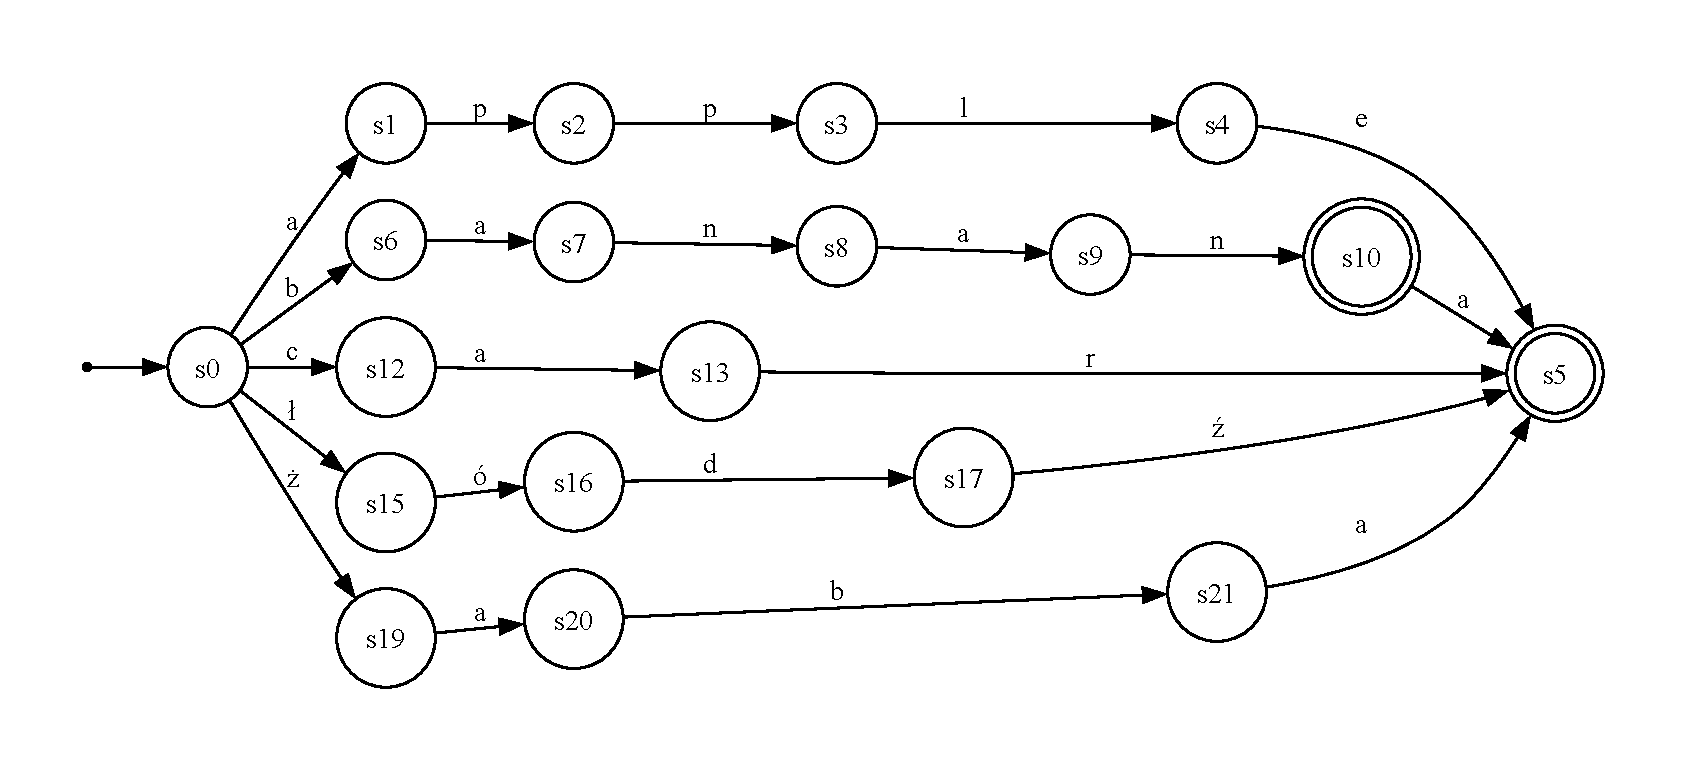
\includegraphics[width=\textwidth]{graphs/example1.pdf}
\end{frame}

\section{Wyniki i ograniczenia}

% Frame 27
\begin{frame}{Metryki diagnostyczne}
    \begin{itemize}
        \item \texttt{stateCount()} -- liczba stanów po finalizacji,
        \item \texttt{reachableStateCount()} -- liczba stanów osiągalnych,
        \item \texttt{transitionCount()} -- liczba przejść,
        \item \texttt{preMinimizationStateCount()} -- stan przed końcową minimalizacją,
        \item \texttt{memoryUsageEstimate()} -- szacowane zużycie pamięci.
    \end{itemize}

    \begin{block}{Uwaga}
        Pomiar pamięci jest estymacją, a nie dokładnym RSS procesu.
    \end{block}
\end{frame}

% Frame 28
\begin{frame}{Demo: mały zbiór danych}
    \begin{itemize}
        \item kilka przykładowych słów: ASCII + polskie znaki,
        \item sprawdzenie działania \texttt{CaseMode},
        \item sprawdzenie obsługi UTF-8,
        \item test iteratora i wyszukiwania,
        \item przykład pomocniczy, nie benchmark wydajności.
    \end{itemize}

    \begin{table}
        \centering
        \small
        \begin{tabular}{lrrr}
            \hline
            Struktura                    & Elementy / stany & Przejścia & Pamięć    \\
            \hline
            Input                        & 7 słów           & --        & 76 B      \\
            \texttt{std::set}            & 7 słów           & --        & 560 B     \\
            \texttt{std::unordered\_set} & 7 słów           & --        & 544 B     \\
            DAFSA przed minimizacją      & 68 stanów        & --        & 10.88 KiB \\
            DAFSA po minimizacji         & 63 stany         & 67        & 3.17 KiB  \\
            \hline
        \end{tabular}
    \end{table}
\end{frame}

% Frame 29
\begin{frame}{Demo na dużym słowniku}
    \begin{table}
        \centering
        \small
        \begin{tabular}{lr}
            \hline
            Metryka                           & Wartość    \\
            \hline
            Liczba słów wejściowych           & 466550     \\
            Liczba unikalnych słów            & 466546     \\
            Liczba znaków                     & 4396435    \\
            Rozmiar wejścia                   & 4.19 MiB   \\
            Stany przed minimalizacją         & 1356532    \\
            Stany po minimalizacji            & 207535     \\
            Przejścia                         & 496498     \\
            Szacowana pamięć po minimalizacji & 13.91 MiB  \\
            Czas budowy                       & ok. 1.91 s \\
            \hline
        \end{tabular}
    \end{table}
\end{frame}

% Frame 30
\begin{frame}{Efekt minimalizacji}
    \begin{table}
        \centering
        \small
        \begin{tabular}{lrr}
            \hline
            Etap                & Liczba stanów & Szacowana pamięć \\
            \hline
            Przed minimalizacją & 1356532       & 104.86 MiB       \\
            Po minimalizacji    & 207535        & 13.91 MiB        \\
            \hline
        \end{tabular}
    \end{table}

    \vspace{0.3cm}

    \begin{block}{Wniosek}
        Liczba stanów spada ponad sześciokrotnie.
    \end{block}
\end{frame}

% Frame 31
\begin{frame}{Porównanie z kontenerami standardowymi}
    \begin{itemize}
        \item \texttt{std::set<std::string>} i \texttt{std::unordered\_set<std::string>}:
              \begin{itemize}
                  \item przechowują słowa jako osobne napisy,
                  \item są uniwersalne i łatwe w użyciu.
              \end{itemize}

        \item \texttt{Lexicon}:
              \begin{itemize}
                  \item nie przechowuje każdego słowa jako osobnego stringa,
                  \item reprezentuje cały zbiór jako automat,
                  \item współdzieli wspólne fragmenty słów.
              \end{itemize}
    \end{itemize}

    \begin{block}{Kiedy DAFSA ma sens?}
        Standardowe kontenery przechowują osobne stringi; Lexicon przechowuje wspólną strukturę automatu. Ma to sens dla dużych, statycznych słowników.
    \end{block}
\end{frame}

% Frame 32
\begin{frame}{Ograniczenia projektu}
    \begin{itemize}
        \item wejście musi być posortowane zgodnie z trybem normalizacji,
        \item brak dynamicznego \texttt{insert} / \texttt{erase} po finalizacji,
        \item tryb \texttt{CaseMode} wybierany jest przed budową automatu,
        \item brak pełnego Unicode case folding,
        \item pomiary pamięci są estymacją,
        \item iterator zwraca słowa kanoniczne, a nie oryginalną pisownię.
    \end{itemize}
\end{frame}

\begin{frame}{Możliwe dalsze kroki}
    \begin{itemize}
        \item pełniejszy benchmark na różnych słownikach,
        \item serializacja gotowego automatu do pliku,
        \item wyszukiwanie prefiksowe i autouzupełnianie,
        \item pełne Unicode case folding przez ICU,
        \item dokładniejsze pomiary pamięci.
    \end{itemize}
\end{frame}

\begin{frame}{Podsumowanie}
    \begin{itemize}
        \item \texttt{Lexicon} publicznie zachowuje się jak kontener słów,
        \item wewnętrznie używa minimalnego automatu acyklicznego,
        \item obsługuje UTF-8, tryby \texttt{Sensitive}/\texttt{Insensitive} i eksport DOT,
        \item minimalizacja redukuje liczbę stanów na dużym słowniku,
        \item projekt pokazuje praktyczne zastosowanie DAFSA w C++20.
    \end{itemize}
\end{frame}

\frame{\maketitle}
\end{document}